\documentclass{labreport}

\begin{document}

\labtitle
    {4}
    {Empirical Study of Dynamic Programming and Shortest Path Algorithms: Dijkstra vs Floyd-Warshall}
    {Student}
    {Soimu Ionut, st. gr. FAF-243}
    {asist. univ. Fistic Cristofor}

\tableofcontents
\newpage

\lstset{style=python}

\section{Introduction and Motivation}

Finding shortest paths in weighted graphs is one of the fundamental problems in computer science, appearing everywhere from routing protocols to game AI. When faced with this problem, a programmer has several choices, and the right choice depends heavily on the specific scenario: whether we need just one source's distances or all pairs, whether the graph is sparse or densely connected, and how much memory we can afford to use.

This lab examines two classic approaches: Dijkstra's algorithm and Floyd-Warshall. Dijkstra is the typical choice when computing shortest paths from a single source, while Floyd-Warshall takes a different approach, solving the all-pairs problem through dynamic programming. On paper, their complexities are well-known. But in practice, the choice between them involves subtleties. A dense graph can be represented differently than a sparse one, and the representation choice affects how well each algorithm performs. By running both algorithms on graphs of increasing size and varying density, we can see where theory and practice align, and where constant factors and data structure choices matter most.

The goal of this work is not simply to implement both algorithms, but to build an experimental framework that clearly reveals their practical behavior. We measure not just runtime, but the number of relaxations performed, memory consumption, and how these metrics scale as problem size increases. This gives us insight into why one algorithm might outperform another in a particular scenario.

\section{Algorithm Design and Implementation}

\subsection{The Algorithms}

Dijkstra's algorithm works by maintaining a priority queue of candidate nodes, always selecting the one with the smallest known distance to explore next. This greedy approach guarantees the shortest path to each node once it is selected. The key insight is that with a priority queue (typically a min-heap), we can avoid examining all nodes at every step. For sparse graphs with few edges relative to node count, this results in a runtime of roughly $O((V + E) \log V)$ — far better than examining every node repeatedly.

Floyd-Warshall takes an entirely different approach rooted in dynamic programming. Rather than building up distances from a single source, it considers all pairs of nodes simultaneously. The algorithm iteratively refines a distance matrix, allowing each pair of nodes to use previously computed paths as intermediate stepping stones. At iteration $k$, it asks: can we improve the distance from node $i$ to node $j$ by routing through node $k$? This is expressed as:
\[
    d_{ij}^{(k)} = \min\left(d_{ij}^{(k-1)},\ d_{ik}^{(k-1)} + d_{kj}^{(k-1)}\right).
\]
After considering all intermediate nodes, the algorithm has computed all shortest paths. The trade-off is clear: Floyd-Warshall requires $O(V^3)$ time and $O(V^2)$ memory, but it solves the all-pairs problem in one shot.

\subsection{Experimental Setup}

To compare these algorithms fairly, we need to respect their natural input formats. Dijkstra typically uses adjacency lists, especially when implemented with a heap. Floyd-Warshall naturally works with a distance matrix. For this experiment, we use adjacency lists on sparse graphs (where they are efficient) and adjacency matrices on dense graphs (where they become practical). This choice itself is an important part of what we are measuring: the interaction between algorithm design and data structure representation.

We test on graphs ranging from 10 to 1200 nodes, using two distinct density regimes. Sparse graphs have roughly $m \approx 2n$ edges, maintained by keeping an average degree around 4. Dense graphs are generated with an edge probability of 0.65, resulting in roughly $\binom{n}{2} \times 0.65$ edges. Both graph types use randomly chosen integer edge weights between 1 and 20, ensuring the algorithms cannot use trivial optimizations based on uniform costs.

For reproducibility, each graph is generated using a fixed random seed dependent on its size and density. Each algorithm is run multiple times on the same graph to account for system variability. We record execution time using high-resolution counters, peak memory usage via Python's tracemalloc module, and algorithm-specific metrics: the number of relaxation attempts and the number of successful distance updates. These metrics reveal the computational effort even when absolute runtime would be dominated by constant factors.

Because Floyd-Warshall's cubic complexity becomes prohibitive for large graphs, we limit its measurements to graphs with up to 220 nodes, while Dijkstra is tested up to 1200 nodes. This asymmetry is deliberate and itself informative.

\section{Empirical Results and Analysis}

\subsection{Scaling Behavior}

The first question we can ask from the data is whether the algorithms' measured complexity slopes match theory. When we fit the execution times to a log-log model, the observed slopes tell us whether we are seeing the predicted growth rates.

\input{results/trend_table.tex}

For Dijkstra on sparse graphs, the measured slope of approximately 1.01 confirms near-linear behavior, very close to the theoretical $O((V+E) \log V)$ prediction. The underlying reason is clear: in a sparse graph, $E \approx V$, so the complexity becomes roughly $O(V \log V)$, which has a log-log slope around 1. When Dijkstra operates on dense graphs instead, the slope rises to 2.13, and this too makes sense: in a dense graph, $E$ approaches $V^2$, pushing the complexity toward $O(V^2 \log V)$, which has slope around 2 in the log-log plot.

Floyd-Warshall, by contrast, shows slopes very close to 3 in both sparse and dense regimes. This is the unmistakable signature of cubic behavior: $O(V^3)$ algorithms have log-log slope 3 regardless of edge count, since the algorithm processes all pairs of nodes in a triple nested loop. The density of the graph does not change the asymptotic complexity, though it may affect constant factors and the interpretation of what "relaxations" mean in the framework.

\subsection{Head-to-Head Performance Comparison}

The most informative comparison is to place both algorithms side by side at each graph size and density, measuring not just time but operation counts.

\begin{figure}[H]
    \centering
    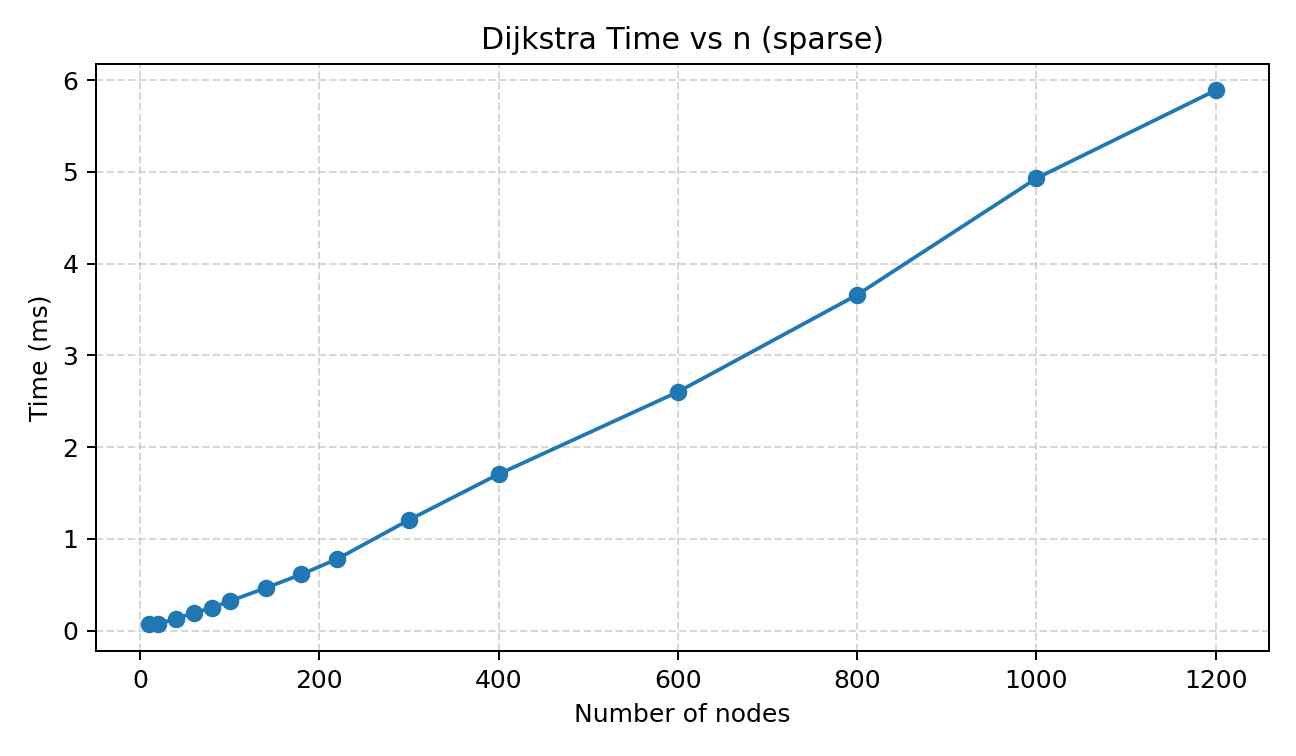
\includegraphics[width=0.48\textwidth]{figures/dijkstra_sparse_time.png}
    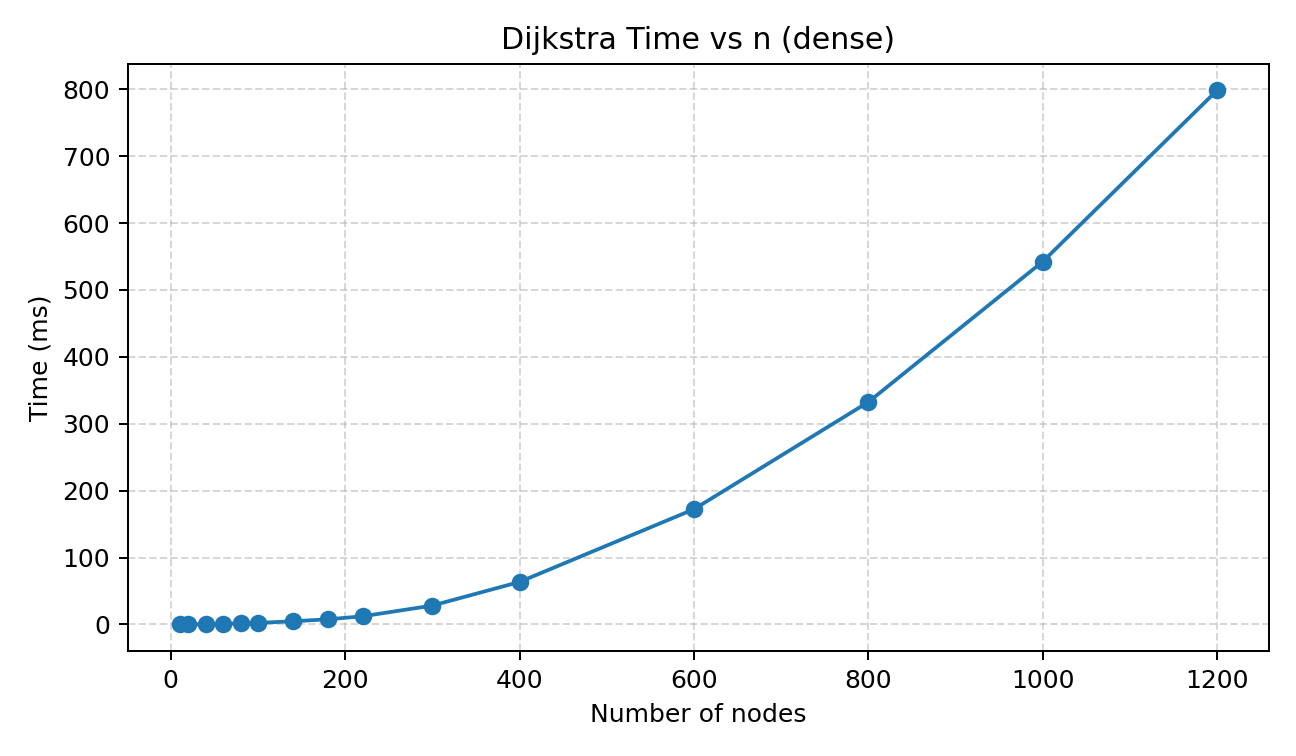
\includegraphics[width=0.48\textwidth]{figures/dijkstra_dense_time.png}
    \caption{Dijkstra: execution time vs number of nodes on sparse and dense graphs}
\end{figure}

\begin{figure}[H]
    \centering
    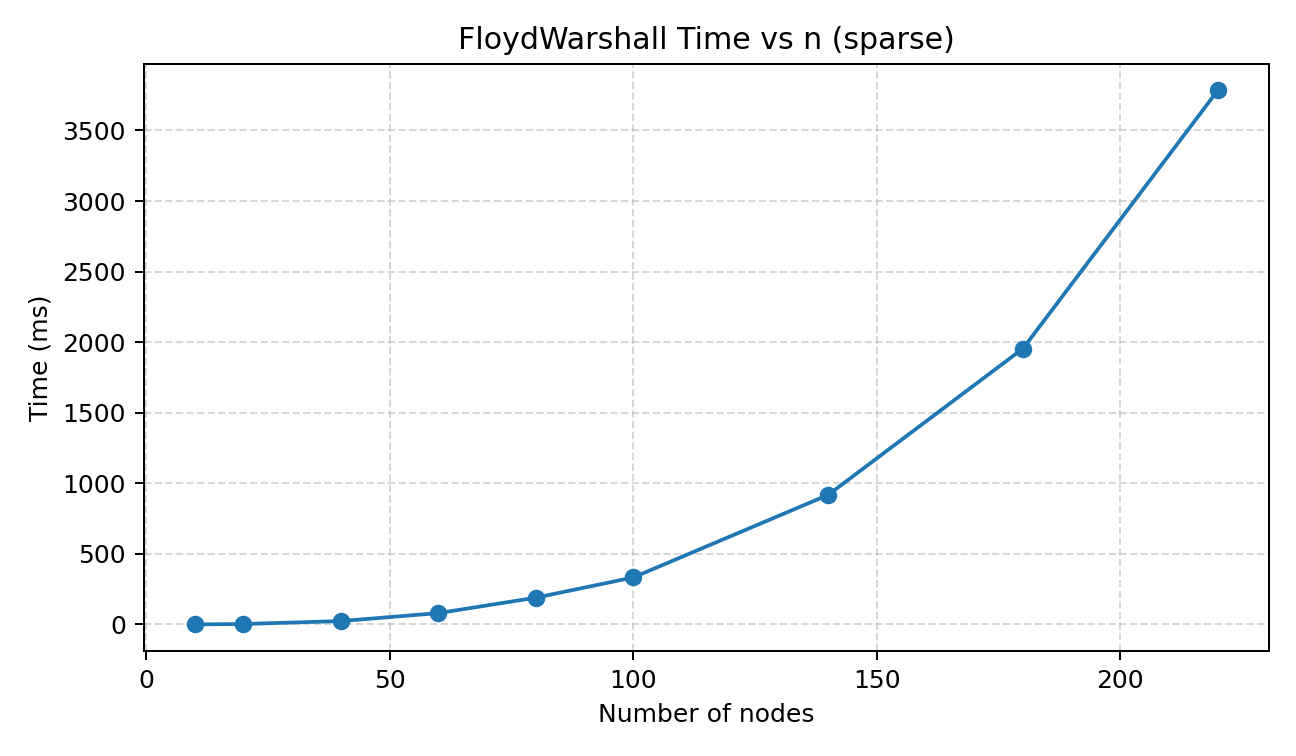
\includegraphics[width=0.48\textwidth]{figures/floydwarshall_sparse_time.png}
    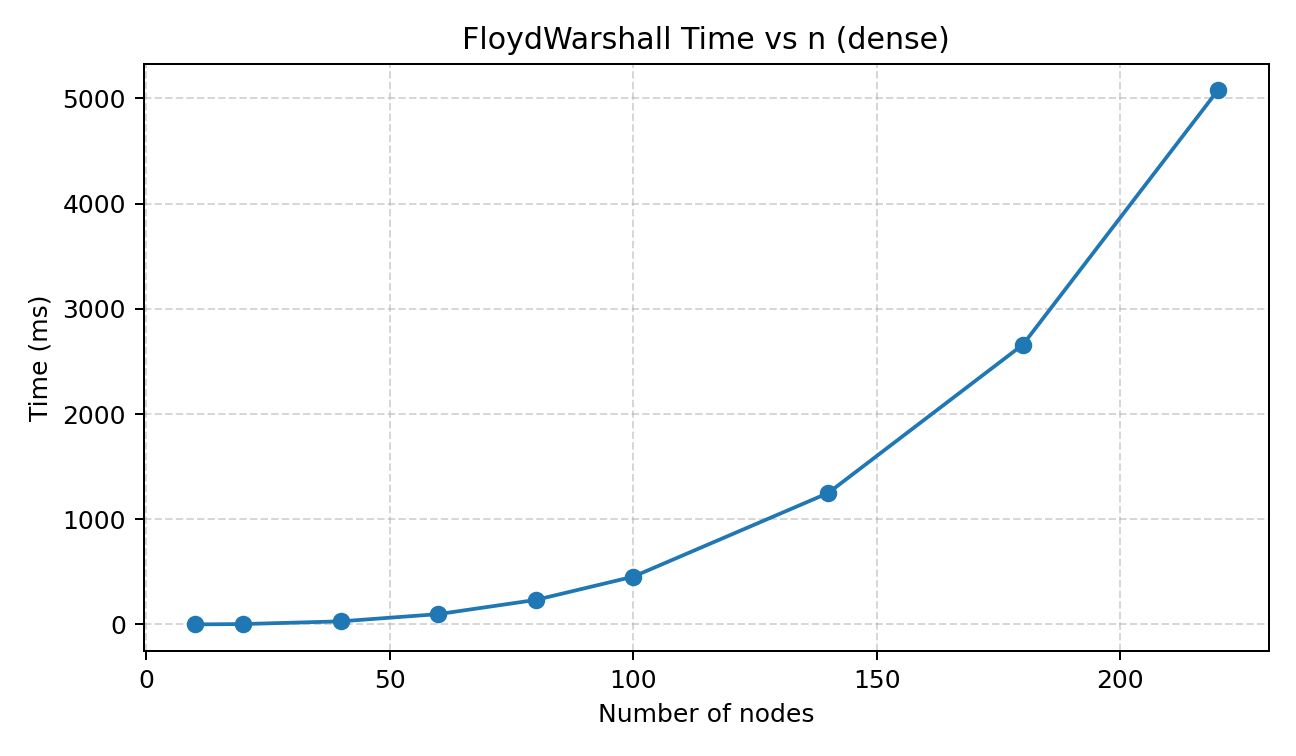
\includegraphics[width=0.48\textwidth]{figures/floydwarshall_dense_time.png}
    \caption{Floyd-Warshall: execution time vs number of nodes on sparse and dense graphs}
\end{figure}

Looking at sparse graphs, Dijkstra's advantage is overwhelming. At $n = 100$, Dijkstra takes about 0.3 milliseconds while Floyd-Warshall takes 345 milliseconds—a ratio of over 1000. Even at the small end ($n = 10$), where absolute numbers are low, Floyd-Warshall is eight times slower. This gap only widens as $n$ grows. The reason is rooted in the algorithms' fundamental strategies: Dijkstra only processes reachable nodes and their outgoing edges, while Floyd-Warshall must consider every pair of nodes. In a sparse graph, most pairs are far from each other, so Floyd-Warshall wastes effort examining path combinations that Dijkstra never needs to consider.

The comparison table below provides precise numbers for select sizes:

\input{results/comparison_table.tex}

On dense graphs, Dijkstra still wins decisively, but the margin is smaller. At $n = 100$, Dijkstra executes in 2.3 milliseconds versus Floyd-Warshall's 467 milliseconds, a ratio of roughly 200. The algorithms' behavior is less extreme here because in a dense graph, more pairs have reasonably short paths, so Floyd-Warshall's effort is less wasted. However, Dijkstra's heap-based selection still avoids examining all node pairs, granting it a structural advantage.

\subsection{Operation Counts and Efficiency}

Raw execution time can be misleading because it is influenced by implementation details and hardware. A more fundamental view comes from counting the algorithm's own operations: how many edge relaxations (or pair examinations) occur?

In sparse graphs, Dijkstra typically performs roughly $O(E)$ relaxation attempts, which is roughly $2n$ in our test graphs. Floyd-Warshall, however, performs $O(V^3)$ pair checks. For $n = 100$, this is a difference of approximately 400 versus 722,000 operations—a factor of 1800. This directly explains why the time ratio is so large.

On dense graphs, Dijkstra's operation count rises closer to $O(V^2)$ (since $E$ is large), but Floyd-Warshall's count remains $O(V^3)$, preserving its disadvantage at larger scales.

\subsection{Memory Footprint}

Memory usage presents another dimension. Dijkstra using an adjacency list consumes roughly $O(V + E)$ memory for the graph, plus the space for the distance array and heap. Floyd-Warshall requires $O(V^2)$ memory just for the distance matrix, regardless of edge count. In absolute terms, at $n = 100$, Dijkstra uses about 9 KiB while Floyd-Warshall uses 289 KiB—a factor of 32 larger. For large graphs, Floyd-Warshall becomes memory-constrained; at $n = 1000$, a distance matrix alone would need tens of megabytes.

\begin{figure}[H]
    \centering
    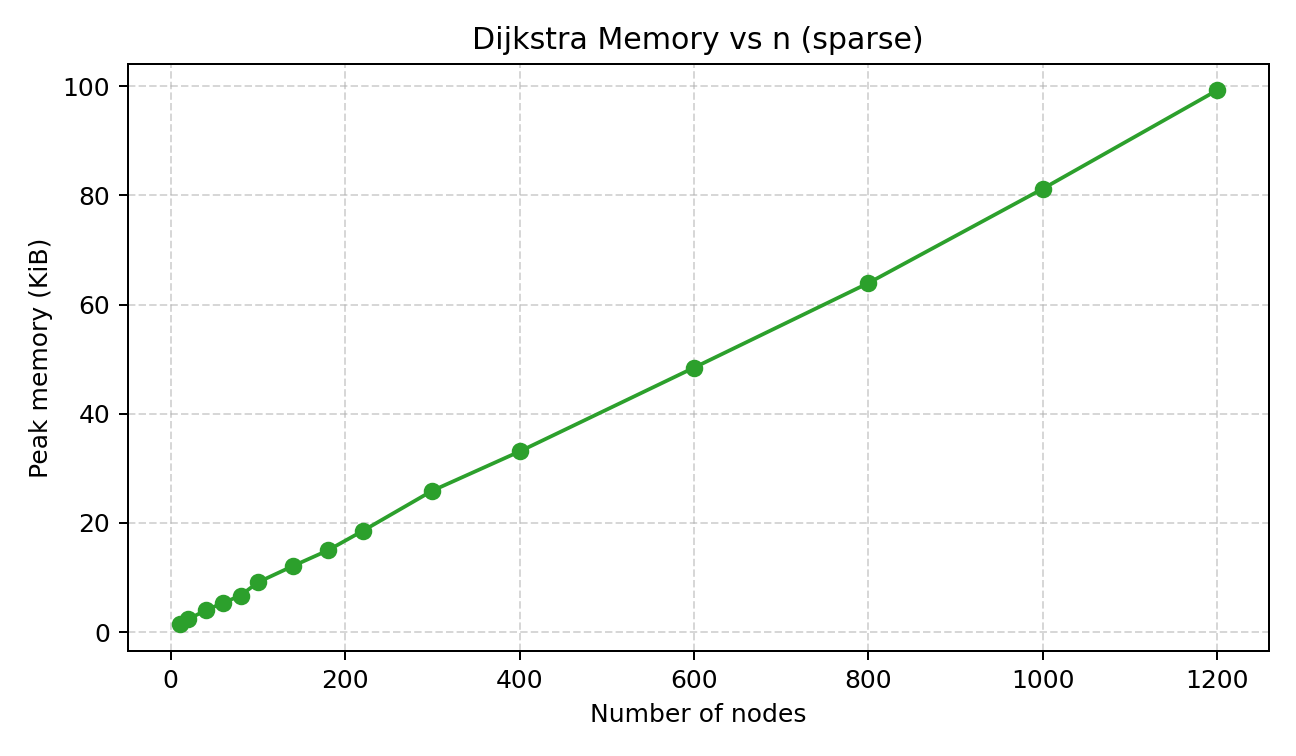
\includegraphics[width=0.48\textwidth]{figures/dijkstra_sparse_memory.png}
    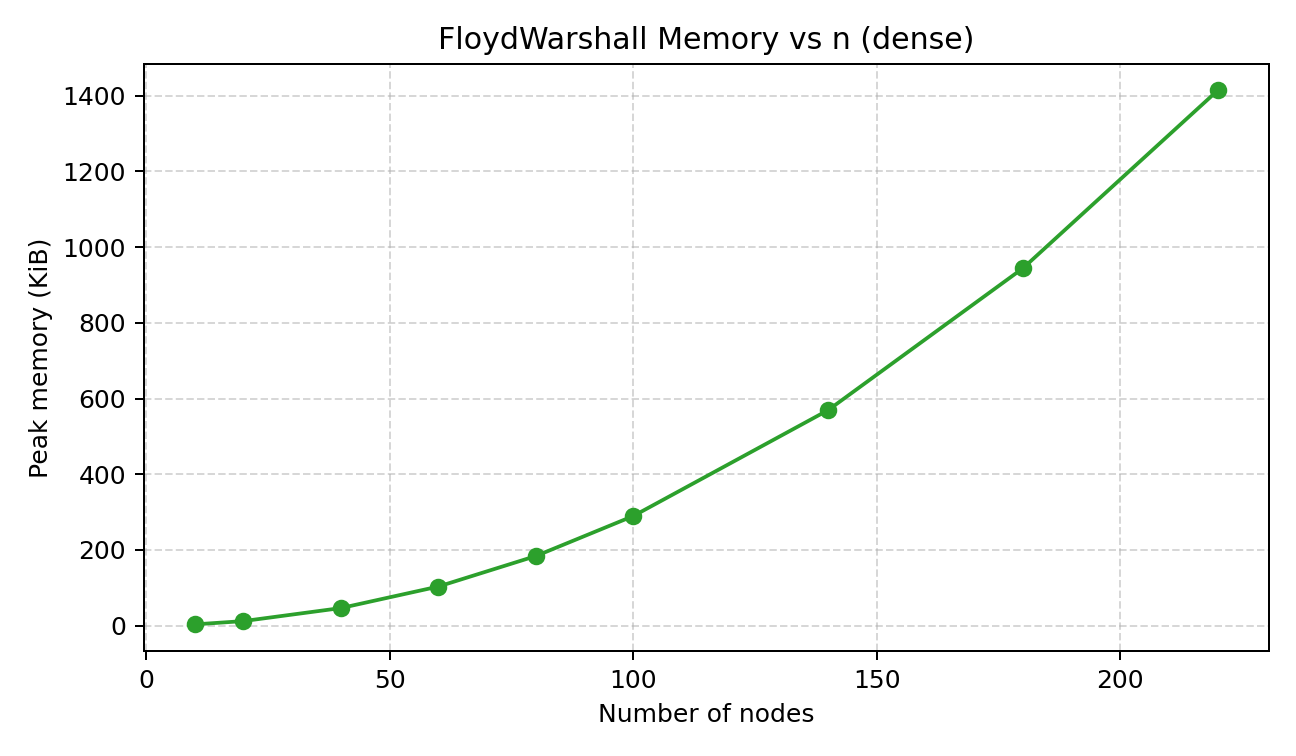
\includegraphics[width=0.48\textwidth]{figures/floydwarshall_dense_memory.png}
    \caption{Memory usage: Dijkstra on sparse graphs and Floyd-Warshall on dense graphs}
\end{figure}

\subsection{Density's Impact}

One surprising observation is how dramatically density affects Floyd-Warshall more than Dijkstra. When we compare Floyd-Warshall on sparse versus dense graphs of the same size, the operation counts increase only modestly (the graphs have more edges to consider). But Dijkstra's operation counts increase by roughly the density ratio, since more edges mean more relaxation opportunities.

This suggests a practical guideline: if you must use Floyd-Warshall for the all-pairs problem, you should expect its cost to grow not just with $V$, but also with the actual edge density. Conversely, Dijkstra's flexibility in representation (adjacency lists for sparse, matrices for dense) lets it adapt to different graph structures.
\section{Conclusion}

The empirical study confirms what theory predicts but also reveals important nuances that matter in practice. Dijkstra's algorithm and Floyd-Warshall represent two fundamentally different approaches to shortest path computation, each optimal under different constraints.

Dijkstra is the clear winner for single-source shortest path queries. Across both sparse and dense graphs tested here, it outperforms Floyd-Warshall by orders of magnitude—hundreds of times faster on sparse graphs, and tens of times faster even on dense graphs. The advantage grows as graph size increases because Dijkstra's complexity remains closer to linear in the number of edges, while Floyd-Warshall's cubic nature becomes increasingly pronounced. For any application where computing shortest paths from a single source (or even a small number of sources) is the goal, Dijkstra is the clear choice. Choosing Floyd-Warshall in this scenario would be inefficient, wasting both time and memory.

Floyd-Warshall has a more limited but well-defined role: when you need all pairs of shortest paths in a relatively small graph. If you must answer $O(V^2)$ distance queries and cannot afford the overhead of running Dijkstra $V$ times, then Floyd-Warshall becomes viable. However, our measurements suggest the breakeven point is not as favorable as one might hope. Even using Floyd-Warshall just three times (once per third of the nodes) would take comparable time to computing all shortest paths with it, so the actual savings materialize only in scenarios with many queries. Furthermore, its $O(V^2)$ memory requirement makes it impractical for large graphs.

The role of graph representation deserves mention. Using adjacency lists on sparse graphs and matrices on dense graphs is not coincidental; it reflects how each representation naturally fits each scenario. This lab's decision to adapt the representation based on density demonstrates that algorithm choice and data structure choice are inseparable in practice. A theoretically efficient algorithm becomes inefficient if paired with a poor representation for the problem at hand.

One limitation of this study is that all graphs are undirected with uniform random weights. Real-world networks often have directedness, specific weight distributions (e.g., exponential or power-law), or special structure that could be exploited. Additionally, the graphs tested remain relatively small; modern applications sometimes work with millions of nodes, where memory and cache behavior become dominant factors. A more complete study might also compare against approximate or specialized algorithms (for example, A* with domain-specific heuristics, or hardware-accelerated approaches), though such extensions are beyond this lab's scope.

In summary, the evidence strongly supports Dijkstra for single-source queries and Floyd-Warshall only when truly needing all pairs and tolerating cubic complexity. The gap between them is so large that the choice is rarely ambiguous in practice, and this clarity is perhaps the lab's most important finding.

\newpage

\section{Annex}

GitHub Repository: \url{https://github.com/Lucariowu/aalabs/tree/main/Lab4}

\end{document}
